\documentclass[border=10pt]{standalone}
\usepackage{tikz}\usepackage{amsmath}\usetikzlibrary{arrows.meta}
\begin{document}
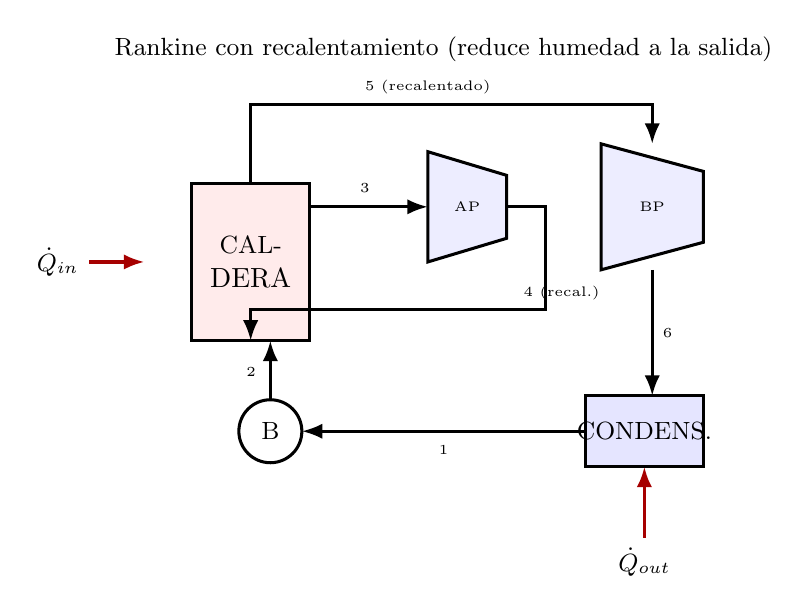
\begin{tikzpicture}[line width=1pt,>={Latex[length=2.6mm]}]
  % caldera con recalentador
  \fill[red!8] (0,1.6) rectangle (1.5,3.6); \draw[line width=1.1pt] (0,1.6) rectangle (1.5,3.6);
  \node[align=center] at (0.75,2.6){\small CAL-\\DERA};
  % turbina AP
  \fill[blue!7] (3.0,2.6)--(4.0,2.9)--(4.0,3.7)--(3.0,4.0)--cycle; \draw[line width=1.1pt] (3.0,2.6)--(4.0,2.9)--(4.0,3.7)--(3.0,4.0)--cycle;
  \node at (3.5,3.3){\tiny AP};
  % turbina BP
  \fill[blue!7] (5.2,2.5)--(6.5,2.85)--(6.5,3.75)--(5.2,4.1)--cycle; \draw[line width=1.1pt] (5.2,2.5)--(6.5,2.85)--(6.5,3.75)--(5.2,4.1)--cycle;
  \node at (5.85,3.3){\tiny BP};
  % condensador
  \fill[blue!10] (5.0,0) rectangle (6.5,0.9); \draw[line width=1.1pt] (5.0,0) rectangle (6.5,0.9);
  \node at (5.75,0.45){\small CONDENS.};
  % bomba
  \draw[line width=1.1pt] (1.0,0.45) circle (0.4); \node at (1.0,0.45){\small B};
  % flujos
  \draw[->,line width=1.1pt] (1.5,3.3)--(3.0,3.3); \node[above] at (2.2,3.35){\tiny 3};
  \draw[->,line width=1.1pt] (4.0,3.3)--(4.5,3.3)--(4.5,2.0)--(0.75,2.0)--(0.75,1.6); \node at (4.7,2.2){\tiny 4 (recal.)};
  \draw[->,line width=1.1pt] (0.75,3.6)--(0.75,4.6)--(5.2,4.6)--(5.85,4.6)--(5.85,4.1); \node[above] at (3.0,4.6){\tiny 5 (recalentado)};
  \draw[->,line width=1.1pt] (5.85,2.5)--(5.85,0.9); \node[right] at (5.85,1.7){\tiny 6};
  \draw[->,line width=1.1pt] (5.0,0.45)--(1.4,0.45); \node[below] at (3.2,0.4){\tiny 1};
  \draw[->,line width=1.1pt] (1.0,0.85)--(1.0,1.6); \node[left] at (0.95,1.2){\tiny 2};
  % interacciones
  \draw[<-,red!65!black,line width=1.2pt] (-0.6,2.6)--(-1.3,2.6); \node[left] at (-1.3,2.6){\small $\dot Q_{in}$};
  \draw[->,red!65!black,line width=1.2pt] (5.75,-0.9)--(5.75,0); \node[below] at (5.75,-0.9){\small $\dot Q_{out}$};
  \node at (3.2,5.3){\small Rankine con recalentamiento (reduce humedad a la salida)};
\end{tikzpicture}
\end{document}
